\section{Detailed Design and Analysis}

The total weight of DynaSaRR with the medkit stowed is approximately 48 lb. In this configuration, the center of mass is 6 in. in front of the back wheel axle and in the center of the chassis (see Fig. \ref{baxle}). 


\subsection{Subsystem Analysis}
Certain sections of the DynaSaRR were identified as subsystems of high import, namely the front wheel forks, the lifting arms, and the medkit arm. These subsystems were chosen due to their propensity to take large impulses and shocks. As such, the SaRRchaeologists determined that if DynaSaRR were to break, it would be at these key points. The following sections represent the analyses of those sections.

\subsubsection{Front Wheel Forks}
The front wheel forks are built from four steel pieces welded together. The HDPE wheel is mounted on an axle supported by the fork (see Fig. \ref{fig:frontforks}). Static and buckling analyses were performed only on the left front wheel fork assembly; as such, only half of DynaSaRR's weight was used for these calculations. Because this subsystem was mirrored across DynaSaRR's center line, the center of mass between the two front wheel forks would simply shift laterally to the center line of DynaSaRR while maintaining the same vertical coordinate.

Figure \ref{fig:displacement} shows that the assembly has a maximum displacement of 1.275e-4 inches. Figure \ref{fig:buckling} shows that a buckling factor of 1948 was predicted by CREO. Based on these simulations, the SaRRchaeologists were able to confidently conclude that the front forks would not be a likely failure mode.

\begin{figure}[hp]
    \centering
    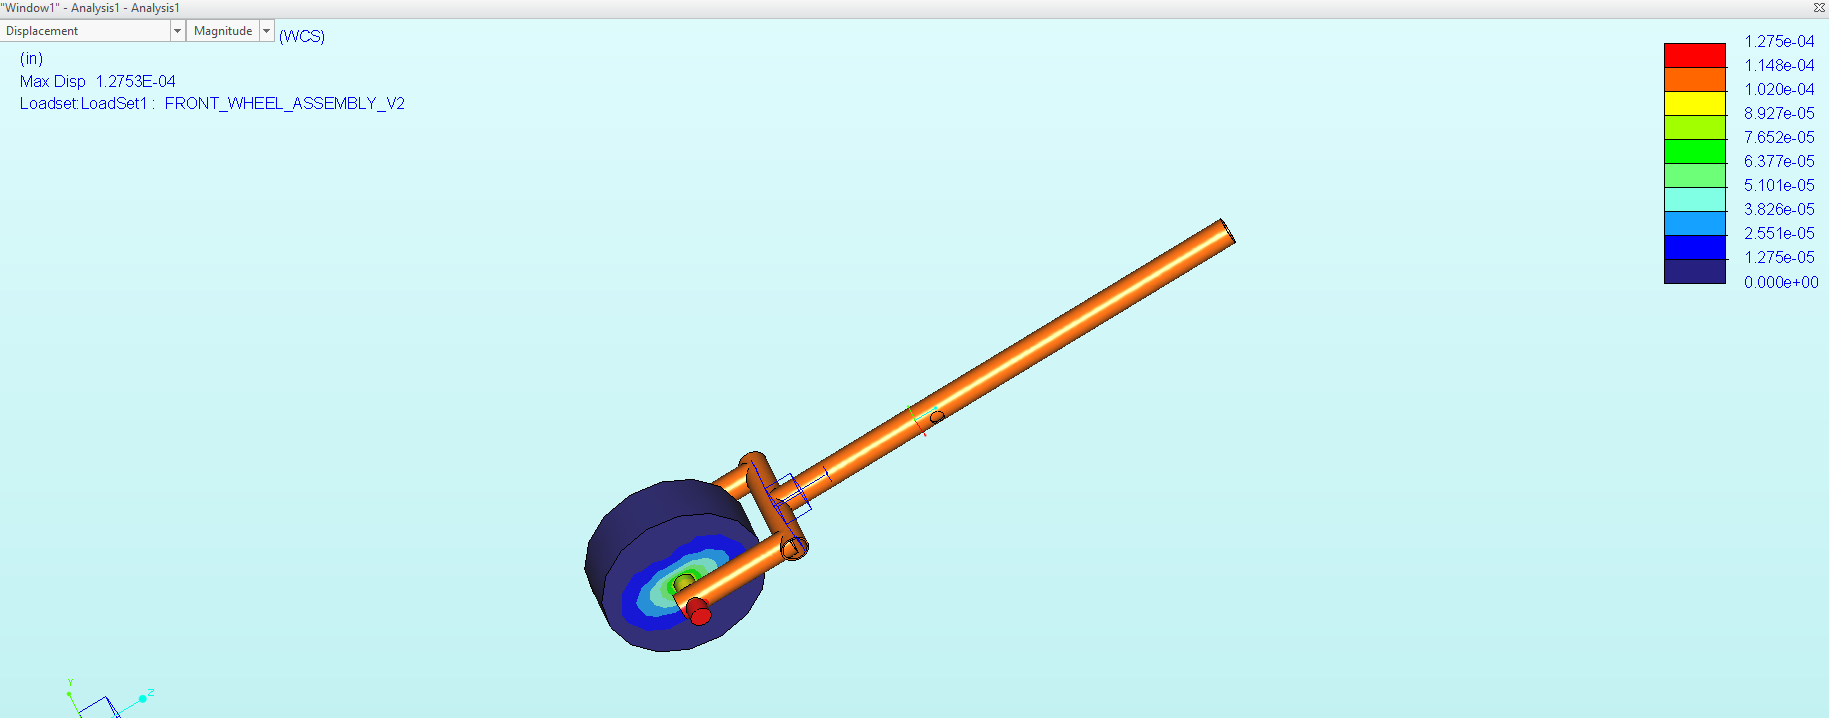
\includegraphics[width=0.4\textwidth]{Images/front_wheel_disp.PNG}
    \caption{Displacement Diagram for Front Wheel Fork Assembly}
    \label{fig:displacement}
\end{figure}
\newpage

\begin{figure}[hp]
    \centering
    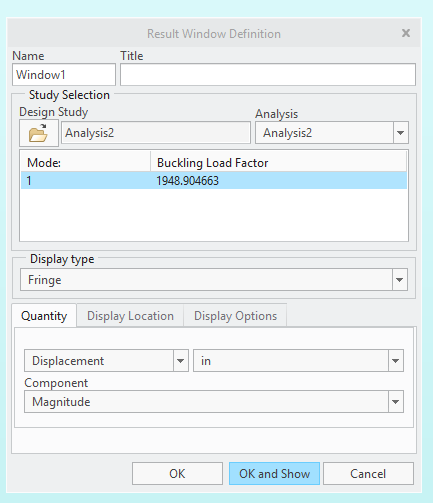
\includegraphics[width=0.4\textwidth]{Images/front_wheel_buckle.PNG}
    \caption{Buckling Factor for Lifting Arm Complex for a load of 25 lbf}
    \label{fig:buckling}
\end{figure}
\newpage

\begin{figure}[hp]
    \centering
    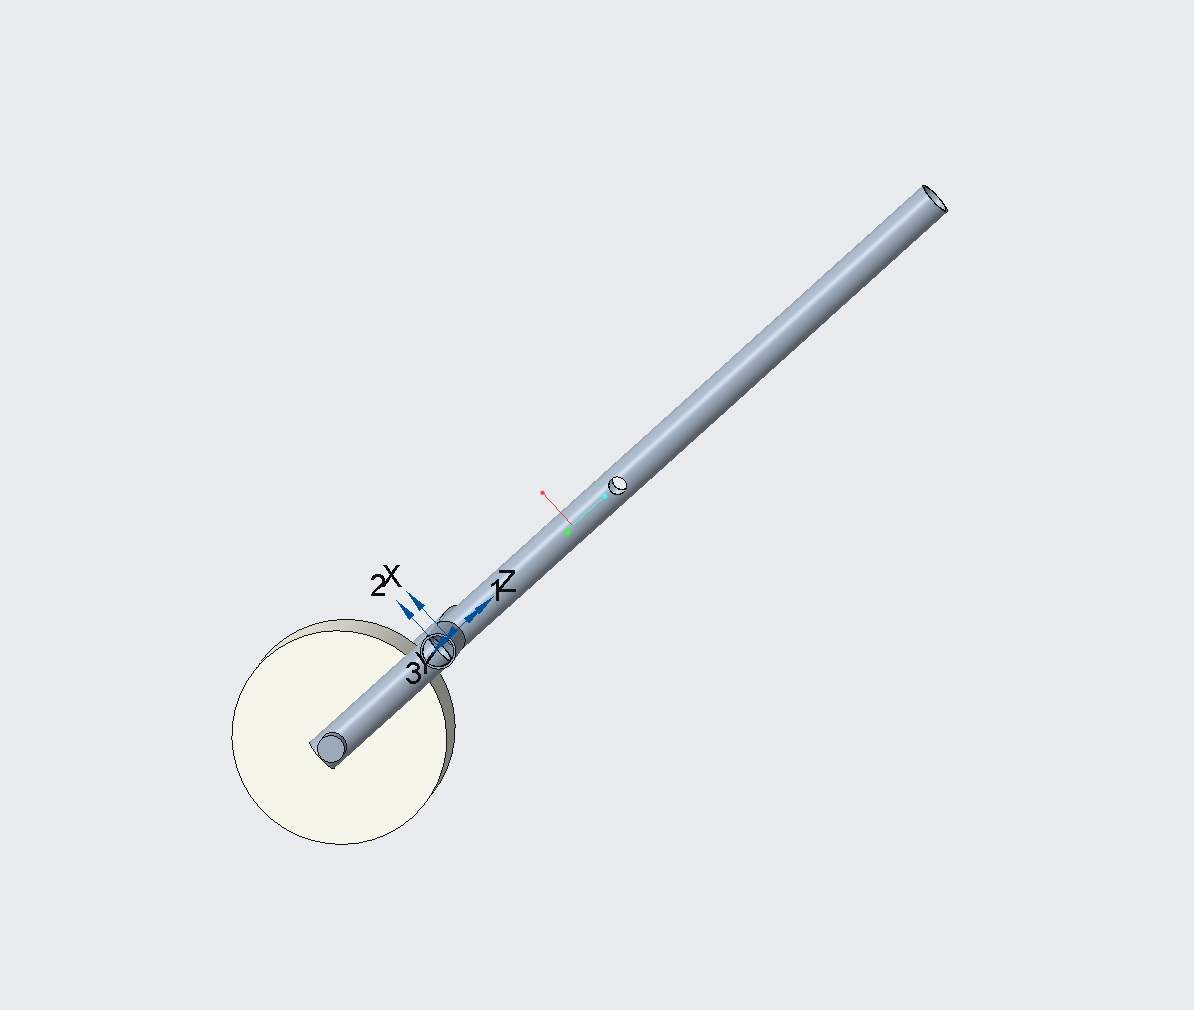
\includegraphics[width=0.4\textwidth]{COM_fork.jpg}
    \caption{Wheel Fork Assembly Center of Mass}
    \label{fig:Center of Mass}
\end{figure}
\newpage


\subsubsection{Lifting Arms}
The lifting arms were made in the CNC from stock HDPE. The gripping plate was also made from an Aluminum 6061 work piece in the CNC. The gripping plate was bolted to the HDPE and then a set screw was used secure it to the axle (for reference, see the Lifting Arm Assembly Drawing in the appendices). Static and buckling analyses were performed on the lifting arm assembly, with only half of DynaSaRR's weight used for these calculations. Because this subsystem was mirrored across DynaSaRR's center line, the center of mass between the two lifting arms would simply shift laterally to the center line of DynaSaRR while maintaining the same vertical coordinate.


Figure \ref{fig:disp2} shows that the assembly has a maximum displacement of .5 inches between the two contact points. Figure \ref{fig:buck2} shows a minimum buckling factor of 4.96. These values show that while the lifting arms were not drastically overengineered, DynaSaRR was unlikely to fail at this point.
\begin{figure}[hp]
    \centering
    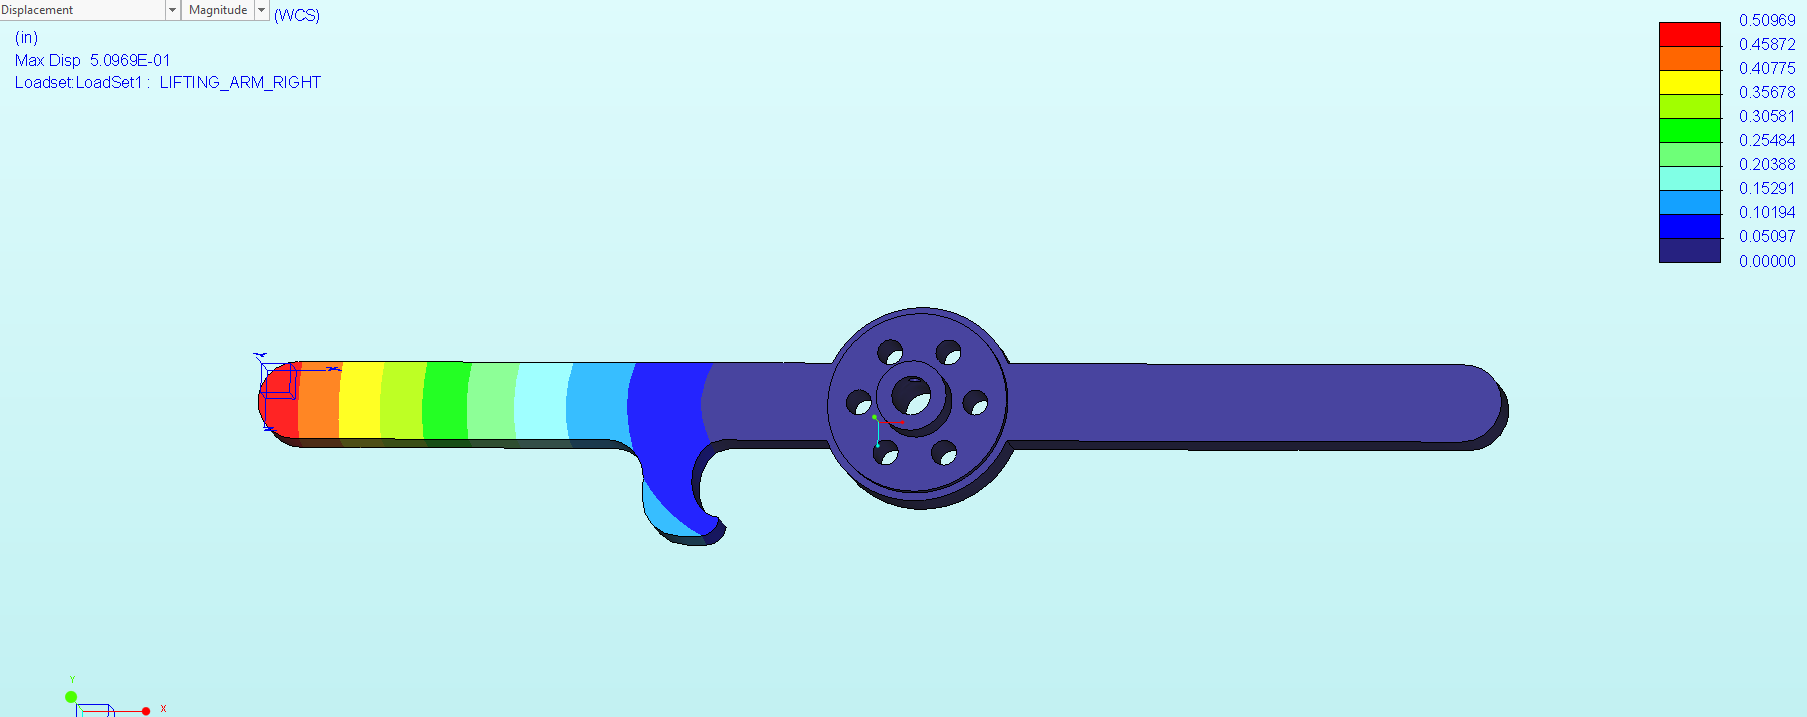
\includegraphics[width=0.5\textwidth]{Images/lifting_arm_final_1_disp.PNG}
    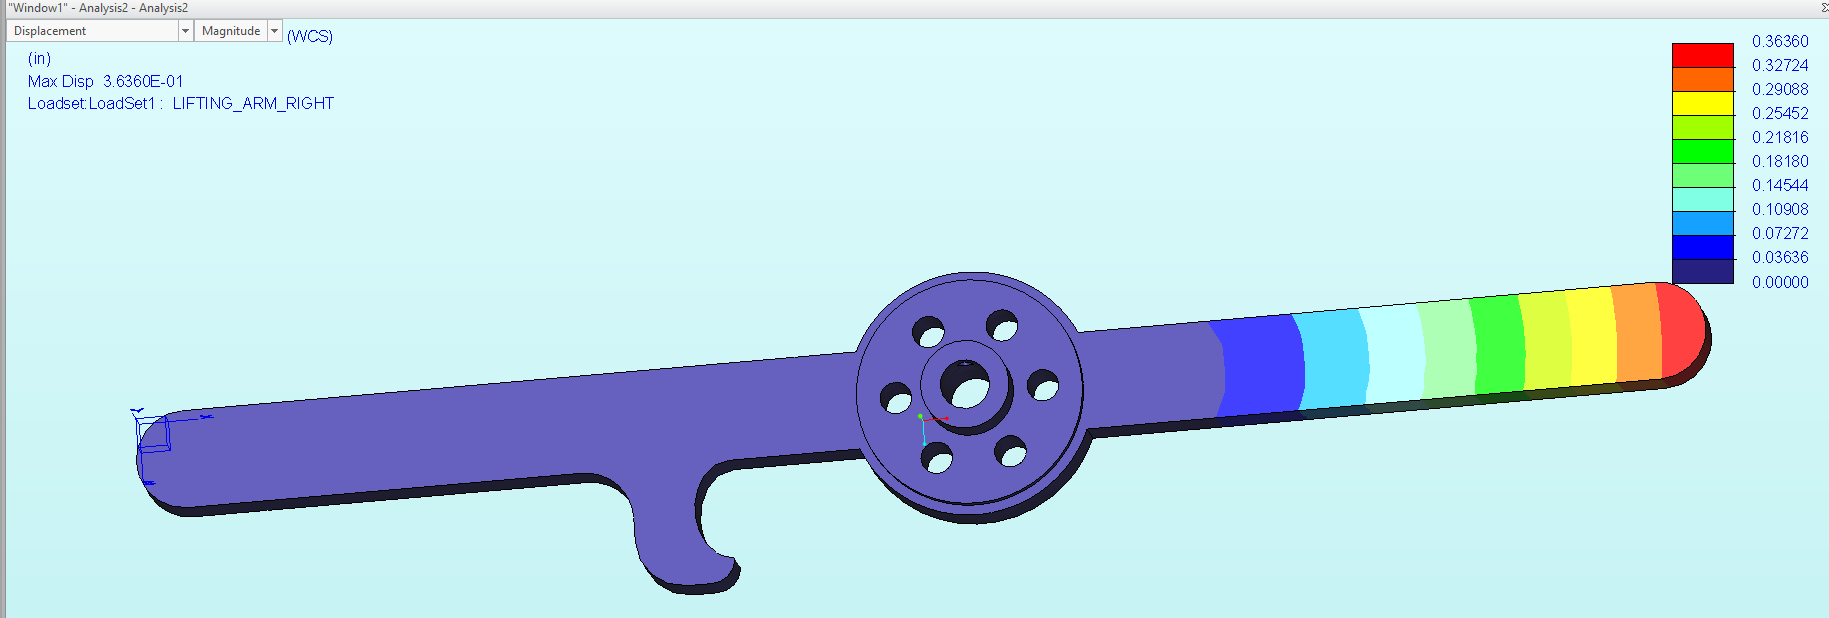
\includegraphics[width=0.5\textwidth]{Images/lifting_arm_final_2_disp.PNG}
    \caption{Displacement Diagram for Lifting Arm Assembly, both points of contact}
    \label{fig:disp2}
\end{figure}
\newpage

\begin{figure}[hp]
    \centering
    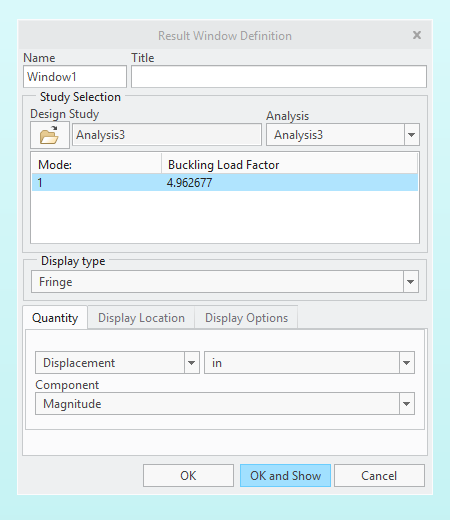
\includegraphics[width=0.25\textwidth]{Images/lifting_arm_final_1_buckle.PNG}
    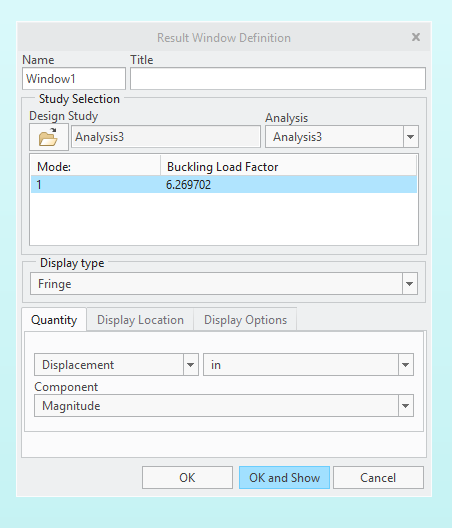
\includegraphics[width=0.25\textwidth]{Images/lifting_arm_final_2_buckle.PNG}
    \caption{Buckling Factor for Lifting Arm Assembly for a load of 25 lbf, both points of contact}
    \label{fig:buck2}
\end{figure}
\newpage

\begin{figure}[hp]
    \centering
    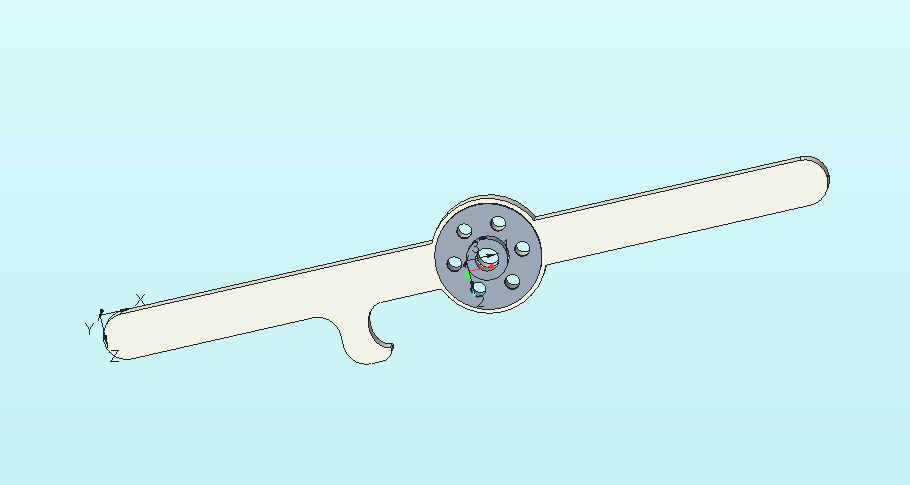
\includegraphics[width=0.5\textwidth]{Capture.PNG}
    \caption{Lifting Arm Assembly Center of Mass}
    \label{fig:FrontFork}
\end{figure}
\newpage

\subsubsection{Medkit Arm}

The Medkit Arm was made from an Aluminum 6061 work piece and an Aluminum 6061 80/20 extrusion. The portion of the arm that grabs the medkit was made in the CNC from a stock Aluminum 6061 piece. The pieces are bolted together (for reference, see Medkit Assembly Drawing). Static and buckling analyses were performed on the Medkit Arm Assembly, with Fig. \ref{fig:disp3} showing a maximum displacement of 0.00366 inches, and Fig. \ref{fig:buck3} showing a buckling factor of 1790.3. These simulations show that this arm was also significantly overengineered for the given medkit, and that it would be virtually guaranteed not to fail.

\begin{figure}[hp]
    \centering
    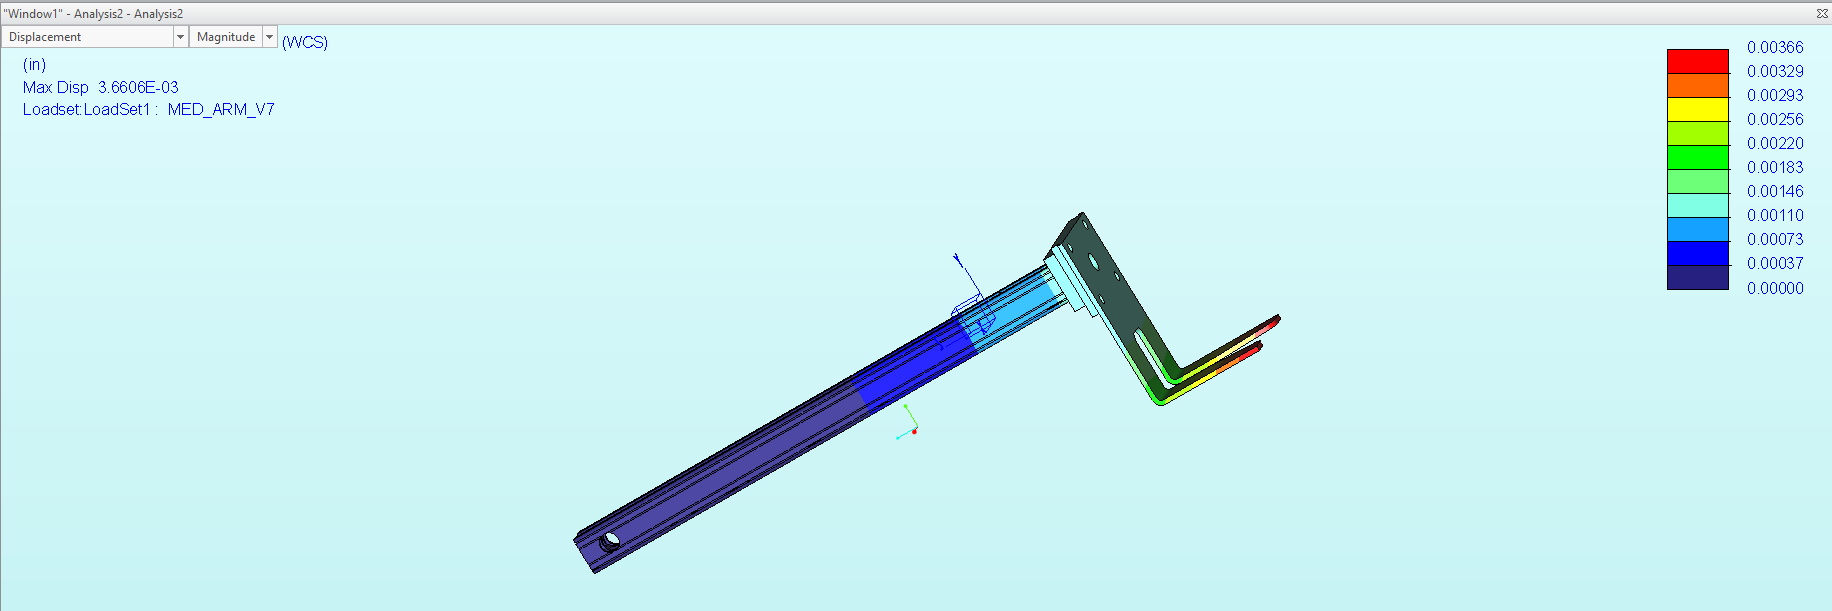
\includegraphics[width=0.4\textwidth]{Images/medkit_displ.PNG}
    \caption{Displacement Diagram for Medkit Arm Assembly}
    \label{fig:disp3}
\end{figure}
\newpage

\begin{figure}[hp]
    \centering
    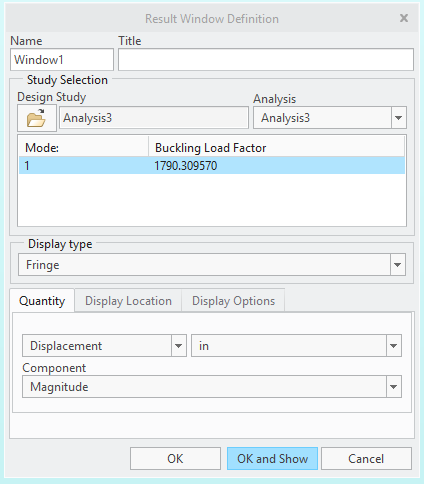
\includegraphics[width=0.4\textwidth]{Images/medkit_buckling.PNG}
    \caption{Buckling Factor for Medkit Arm Assembly for a load of 5 lbf}
    \label{fig:buck3}
\end{figure}
\newpage

\begin{figure}[hp]
    \centering
    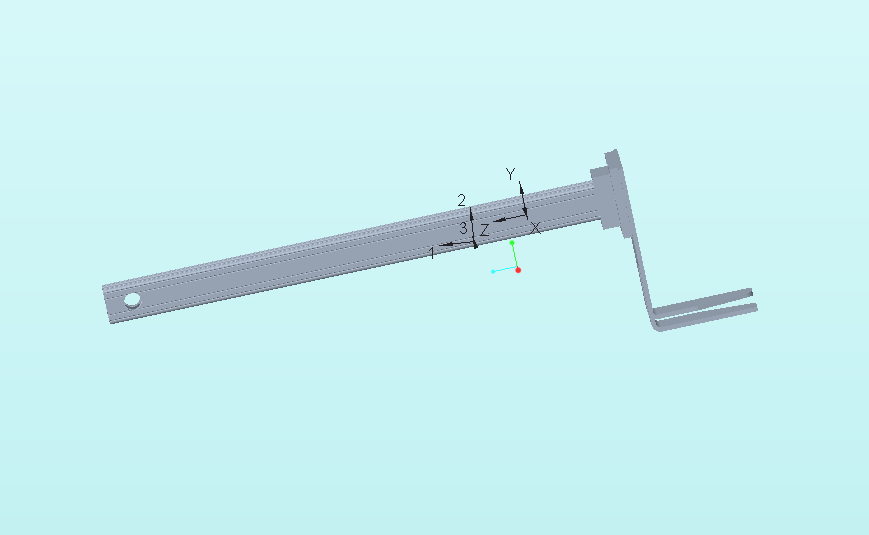
\includegraphics[width=0.5\textwidth]{Images/medkit_COM.PNG}
    \caption{Medkit Arm Assembly Center of Mass}
    \label{fig:MedkitArm}
\end{figure}
\newpage








\begin{figure}[hp]
    \centering
    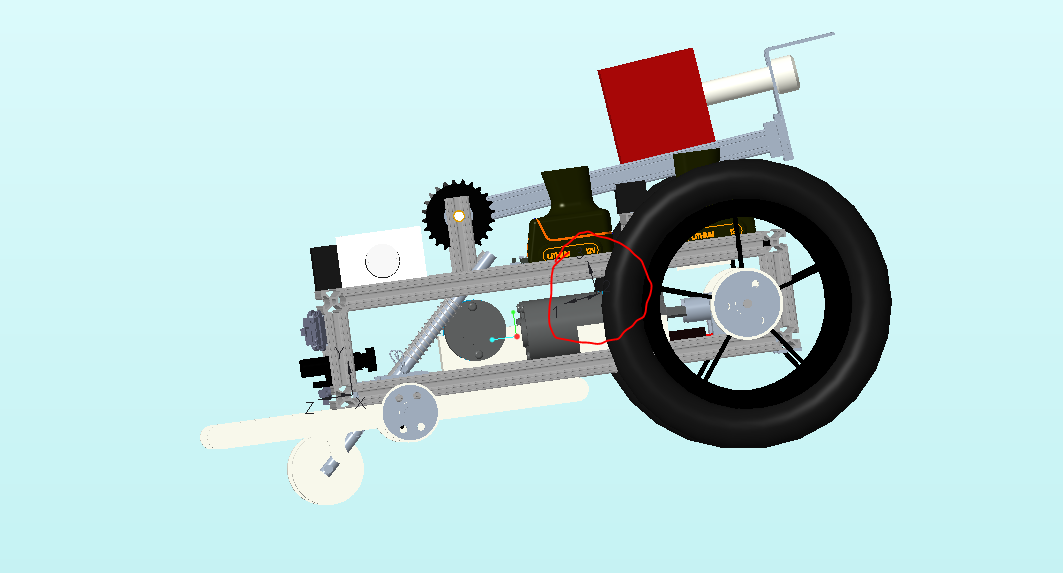
\includegraphics[width=0.8\textwidth]{Images/assemblyCOM.PNG}
    \caption{Fully Assembled DynaSaRR with Isolated Center of Mass}
\end{figure}

The free body diagrams of the configurations mentioned previously are illustrated in figures \ref{fig:analysis1_medkitstowed} and \ref{fig:analysis2_liftingmedkit}.  In both figures, it can be seen that the back of DynaSaRR supports more weight than the front.  This is useful in the medkit retrieval, as the calculations show that it would take a load of 69.3 lb at the end of the medkit arm for DynaSaRR to tip over.

\label{fig:analysis1_medkitstowed}
\begin{figure}[hp]
    \centering
    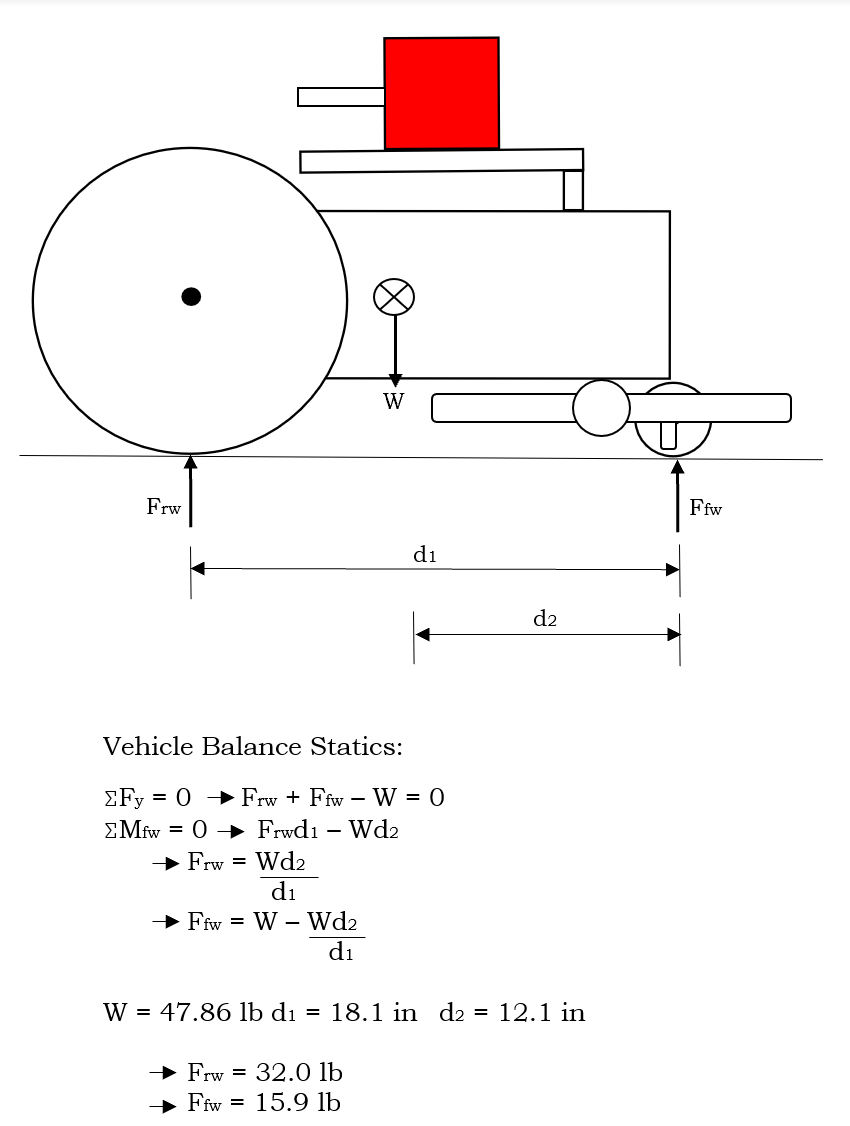
\includegraphics[width=0.8\textwidth]{Images/analysis1_medkitstowed.png}
    \caption{Free Body Diagram and Calculations for DynaSaRR with Med Kit Stowed}
    \label{fig:analysis1_medkitstowed}
\end{figure}
\vfill
\newpage

\label{fig:analysis2_liftingmedkit}
\begin{figure}[hp]
    \centering
    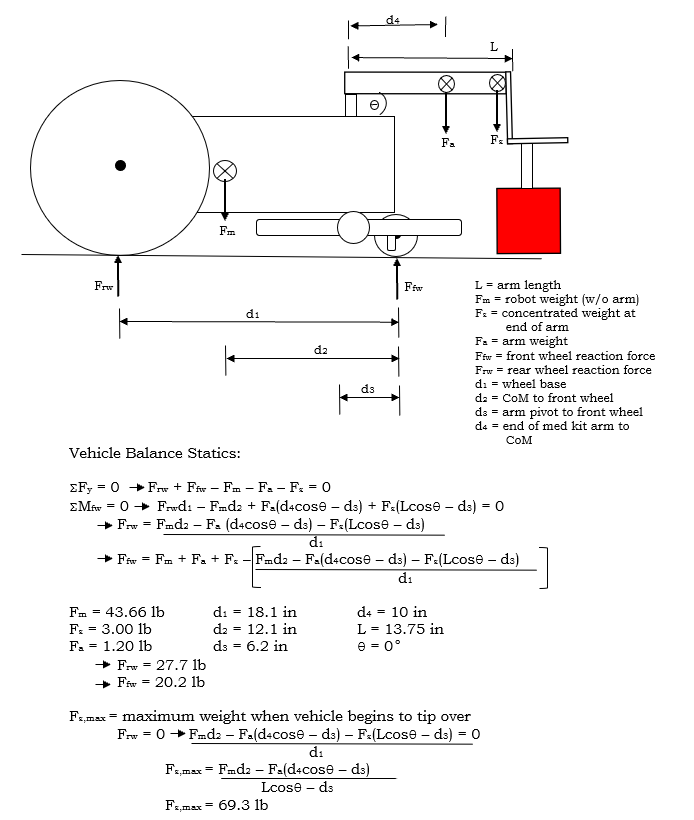
\includegraphics[width=0.8\textwidth]{Images/analysis2_liftingmedkit.png}
    \caption{Free Body Diagram and Calculations for DynaSaRR when Beginning to Lift Med Kit}
    \label{fig:analysis2_liftingmedkit}
\end{figure}
\vfill
\newpage


In designing a medkit retrieval mechanism, the primary considerations were a gripper that would not require tremendous precision in order to pick up the med-kit handle, and a mechanism to secure the med-kit into place after it was lifted onto the SaRR, so that it would not fall out during the wall traversal or other sections of the obstacle course. To fit the first consideration, DynaSaRR lowers an arm with a flat gripper component at the front. The gripper is composed of two triangular pieces of aluminum that funnel the handle of the medkit into the triangular space between them and then into a slot cut into the gripper. The V-shaped gripper is intended to minimize the precision required in driving up to the med-kit by providing a large capture area. The arm then rotates upward, with the med-kit pivoting in the gripper slot until it falls into a bracket mounted on the underside of the arm intended to secure it.

The SaRRchaeologists decided to utilize the same Vex Mini CIM Motor for the lifting arms as was used for the back wheels. The published data shows a stall torque of 1.41 Newton-Meters. The SaRRchaeologists used a conservative estimate of 1.3 Newton-Meters, a gear ratio of 24:1, and equation (1) 
\begin{equation}
    torque_{new} = torque_{original} * gearRatio
\end{equation}
and where able to achieve a theoretical torque of 31.2 newton-meters. This value is equivalent to 23.08 foot-pounds of generated torque. 

Free body diagram analyses were completed on DynaSaRR at different stages of traversing the wall to determine if the lifting arm motor had enough torque for DynaSaRR to successfully clear the wall.  These can be seen in Figures \ref{fig:analysis3_wall1}-\ref{fig:analysis5_wall3}.

In order for the lifting arms to lift the front of DynaSaRR, they must produce a minimum torque of 15.3ft-lb, which was the maximum torque calculated from the different stages of wall traversal as seen in Figure \ref{fig:analysis4_wall2}.  The SaRRchaeologists knew that this torque would be possible with the chosen motor when compared with its generated torque value of 23.08 ft-lb found from equation (1).
\begin{equation}
    torque_{min} = \frac{Wd_{2}d_{3}}{d_{1}} = 15.3 ftlb
\end{equation}

\label{fig:analysis3_wall1}
\begin{figure}[hp]
    \centering
    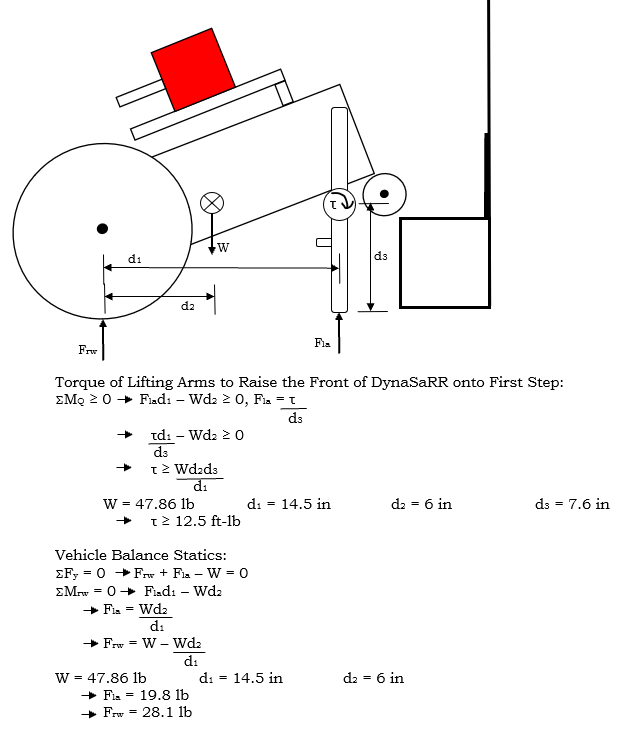
\includegraphics[width=0.9\textwidth]{Images/analysis3_wall1.png}
    \caption{Free Body Diagram and Calculations for DynaSaRR to Traverse Wall- Stage 1}
    \label{fig:analysis3_wall1}
\end{figure}
\vfill
\newpage

\label{fig:analysis4_wall2}
\begin{figure}[hp]
    \centering
    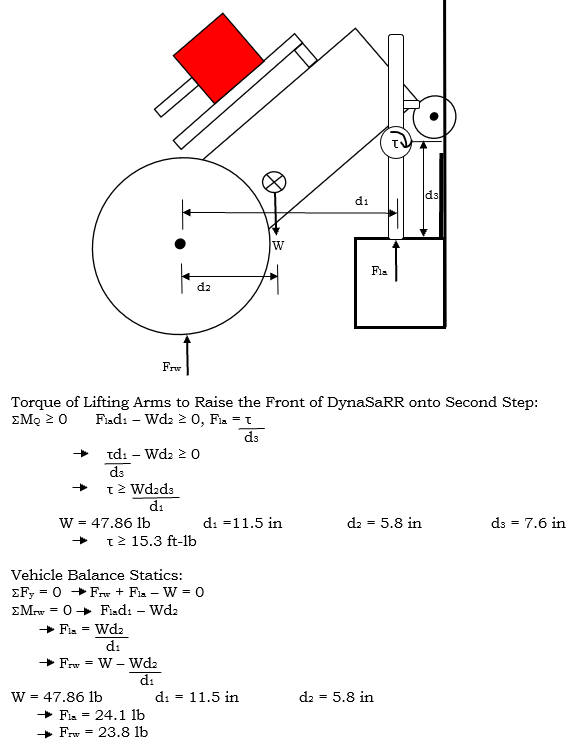
\includegraphics[width=0.7\textwidth]{Images/analysis4_wall2.png}
    \caption{Free Body Diagram and Calculations for DynaSaRR to Traverse Wall- Stage 2}
    \label{fig:analysis4_wall2}
\end{figure}
\vfill
\newpage

\label{fig:analysis5_wall3}
\begin{figure}[hp]
    \centering
    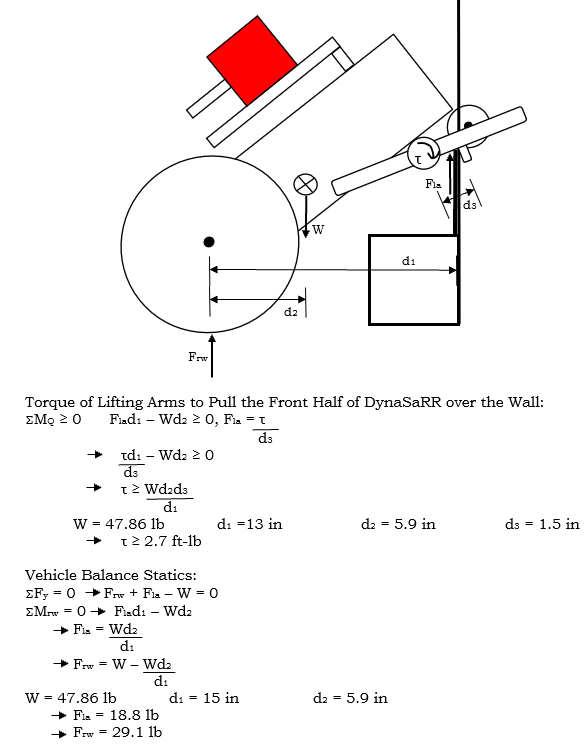
\includegraphics[width=0.7\textwidth]{Images/analysis5_wall3.png}
    \caption{Free Body Diagram and Calculations for DynaSaRR to Traverse Wall- Stage 3}
    \label{fig:analysis5_wall3}
\end{figure}
\vfill
\newpage

Using the the published data, The SaRRchaeologists found that an RPM of 58 was associated with the necessary raw torque of the lifting arm motor, 1.3 newton-meters. Using the 24:1 gearing ratio again and equation (3),

\begin{equation}
    RPM_{new} = \frac{RPM_{original}}{gearRatio} 
\end{equation}


it was calculated that the RPM of the lifting arm would be approximately 4. As such, it would take approximately 22.5 seconds for the lifting arm to rotate 270 \degrees, the estimate required to get it over the wall. However, in practice, the lifting arms were found to rotate faster than this, as the wall traversal took a significantly shorter time (see section 5.1).

To get over the highest point of the wall, the configuration shown below in Figure \ref{fig:analysis6_wall4} illustrated that as long as DynaSaRR's center of mass was to the right of the pivot point, p, DynaSaRR would tip over the wall. 
\begin{equation}
    \sum M_{p} = -W*d<0
\end{equation}
\label{fig:analysis6_wall4}
\begin{figure}[hb]
    \centering
    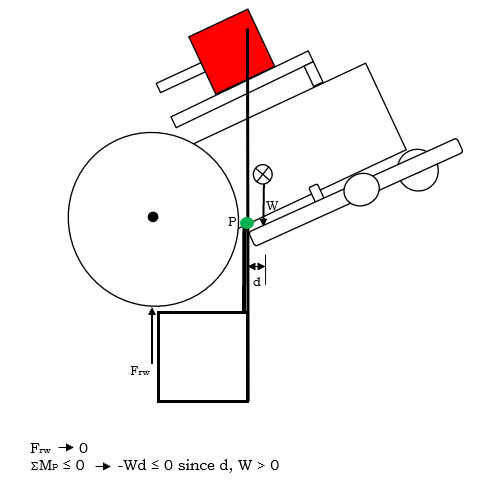
\includegraphics[width=0.6\linewidth]{Images/analysis6_wall4.png}
    \caption{Free Body Diagram and Calculations for DynaSaRR to Traverse Wall- Stage 4}
    \label{fig:analysis6_wall4}
\end{figure}
\vfill
\newpage

When examining static-stability margins, Figure \ref{fig:analysis6_wall4} provides a good demonstration of DynaSaRR's ability to tip over the wall. In this configuration, the center of mass was approximately 0.5 in. in front of the pivot point. This implied that DynaSaRR had just enough weight in front of this point for the front end to fall down, since the distance between the pivot point and the center of mass only had to be greater than zero. Since this measured distance was fairly small, it did not guarantee that the robot would tip over fully on its on, so the lifting arms acted as a secondary tool for the SaRR to traverse the highest point of the wall. The lifting arms pushed against the back of the wall to ensure that the center of mass shifted in front of the pivot point. If the center of mass was shifted further forward, it would be easier for DynaSaRR to tip over the wall. One way this could be achieved would be to shorten the length of the medkit arm. However, the SaRRchaeologists determined that a longer medkit arm was needed in order to deposit the medkit into the basket accurately. While this made completing the final task of the obstacle course easier, it decreased the margin of error during wall traversal. If the center of mass was shifted back by anything greater than 0.5 in., these calculations showed DynaSaRR would not be able to tip over the wall.

The final free body diagram of the wall traversal calculated the force on the front wheels upon dismounting hte walls. The SaRRchaeologists knew that the front wheels would be feel a much greater force compared to their normal driving configuration, since they would be the first part of DynaSaRR to make contact with the ground. Therefore, shocks were added to the front wheels, which were mounted to the chassis with steel forks at a 45\degree angle. The angle allowed for them to be further out from the front of the chassis. This was intended to prevent the front of the chassis from making contact with the ground during any failed trials while testing by stopping the robot's fall earlier. It was found in Figure \ref{fig:analysis7_wall5} that the front wheels experienced a force of 25.8 lbf. Initially, the SaRRchaeologists thought that the front wheels would feel the entire force of DynaSaRR's weight. However, after watching multiple videos of DynaSaRR traversing the wall and creating different free body diagram configurations, it was noted that the back wheels remained in contact with the wall when the front wheels first made contact with the ground. Therefore, the front wheels experienced less force than previously expected, but the shocks remained useful in preventing the sudden impact from damaging more sensitive parts of the assembly.

\label{fig:analysis7_wall5}
\begin{figure}[hb]
    \centering
    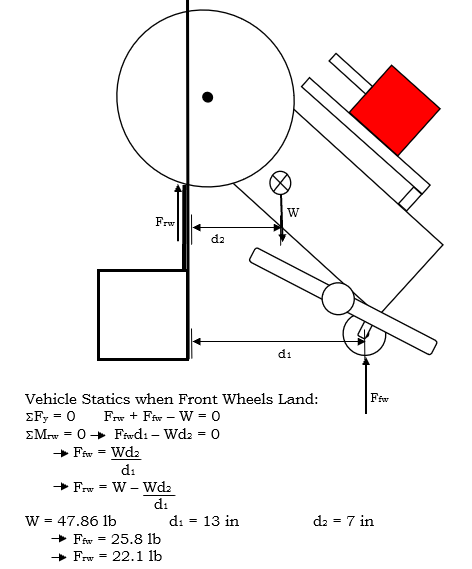
\includegraphics[width=0.7\linewidth]{Images/analysis7_wall5.png}
    \caption{Free Body Diagram and Calculations for DynaSaRR to Traverse Wall- Stage 5}
    \label{fig:analysis7_wall5}
\end{figure}
\vfill
\newpage
\clearpage

\subsection{Control Algorithm}
1- Block Diagrams

In open-loop mode, each of the robot's functions is assigned to a lever on the controller. The value outputted by the controller is proportionally mapped to the range of each motor driver, which then sends the appropriate signal to the motor to complete the action.


Once switched into autonomous mode, DynaSaRR first checks if the wall has been cleared. This condition can be triggered by either a) completing the wallTraverse function, or b) being manually marked as completed using the left switch on the remote. If it is still marked as false, it goes into the wallTraverse function, which gives 25 \percent forward power to the rear wheels and 75 \percent forward power to the lifting arms until the robot has climbed the two steps and has its front wheels hooked over the top of the wall. It then gives full forward power to the wheels and lifting arms in order to pull the robot over the wall. Having completed this part of the course, and with the wall marked as cleared, DynaSaRR goes into chute traversal mode. It reads the difference between the two proximity sensors placed on either side of the front of the frame, and turns slightly away from whichever wall is closer. Between readings, it drives slightly forward to ensure that it does not get stuck oscillating back and forth between the walls without making progress. Upon exiting the chute, light tracking is activated, with the code reading the difference in brightness between the two light sensors mounted on the front crossbar and pointed inward so that each one's field of view overlaps the other's. The algorithm turns the robot to the side with the dimmer reading (i.e., if the left light sensor, which points slightly right across the front of the robot, reads a brighter value, the robot will turn slightly to the right to re-enter the column of light) and drives forward when both sensors read approximately equal values, i.e., when the robot is facing directly into the light. Should DynaSaRR turn too far out of the light column and the light signal drop too low, it begins to rotate slowly to the right until it is able to reacquire the signal. Finally, once the proximity sensor mounted to the front of the frame detects the presence of the medkit deposit basket, the robot stops driving and brings the medkit arm forward to place the medkit in the basket.